\documentclass{article}
\usepackage[utf8]{inputenc}
\usepackage{amsmath}
\usepackage{graphicx}

\title{Discussion Assignment}
\author{Jasper Albert Nri}
\date{September 2021}

\begin{document}

\maketitle

\section*{Introduction}
$${x^2 + (y-2)^2 = 1}$$
\begin{itemize}
    \item \textbf{Does the equation determine a relation between ${x}$ and ${y}$} \\
    Yes the above equation clearly depicts a relationship between ${x}$ and ${y}$, with ${(x,y)}$ being points on a circle of radius 1 and center ${(0,2)}$.
    

    \item \textbf{Can the variable ${x}$ be seen as a function of ${y}$\\
    Yes it can} \\
    This can be achieved by making ${x}$ the subject of the equation given above. we can express ${x}$ as a function of ${y}$ like ${x = g(y)}$
    
    $${x^2 + (y-2)^2 = 1}$$
    
    Subtracting ${(y-2)^2}$ from both sides
    $${x^2 = 1 - (y-2)^2}$$
    
    Next, we take the Square root of both the LHS and RHS
    $${x = \pm\sqrt(1 - (y-2)^2)}$$
    
    Once this has been done we are left with an expression of ${x=g(y)}$
    and this expresses ${x}$ as a function of ${y}$, because for any value of ${y}$ placed into the equation $${x = \pm\sqrt(1 - (y-2)^2)}$$ there would be an equivalent value of ${x}$ gotten from it.
    
    
    \item \textbf{Can the variable ${y}$ be seen as a function of ${x}$\\
    Yes it can}\\
    Just like with the variable ${x}$, ${y}$ can also be seen as a function of ${x}$
    we can achieve this by making ${y}$ the subject of the equation
    $${x^2 + (y-2)^2 = 1}$$
    and we start by subtracting  ${x^2}$ from both sides of the equation
    
    $${(y-2)^2 = 1 - x^2}$$
    
    Next we open the brackets on the LHS by taking the square root of both the LHS and the RHS
    
    $${y-2 = \sqrt{1 - x^2}}$$
    
    We then add 2 to both sides, so that we are left with expression
    
    $${y = 2 \pm\sqrt{1 - x^2}}$$
    
    And this equation satisfies the expression of ${y=h(x)}$
    and proves that the variable ${y}$ can be seen as a function of ${x}$
    
    \item \textbf{What will be the domain for these two functions? 
    For the First function that expresses ${x}$ as a function of ${y}$,}\\
    The domain would be
    $${1-(y-2)^2 \ge 0}$$
    $${(y-2)^2 \le 1}$$
    $${{y-2\le\pm\sqrt{1}}}$$
    $${-1 < y-2 <1}$$
    Therefore the domain for this equation is $${1 < y < 3}$$
    
    
    For the Second function that expresses ${y}$ as a function of ${x}$,\\
    The domain would be
    $${1-x^2 \ge 0}$$
    $${x^2 \le 1}$$
    $${{x\le\pm\sqrt{1}}}$$
    $${-1 \le x \le 1}$$
    Therefore the domain for this function is $${-1\le x \le 1}$$

    \item \textbf{What are the graphs of these two functions?\\
    For the function that expresses ${x}$ as a function of ${y}$ i.e}
    $${x=g(y)}$$
    
    The graph is seen below\\    
    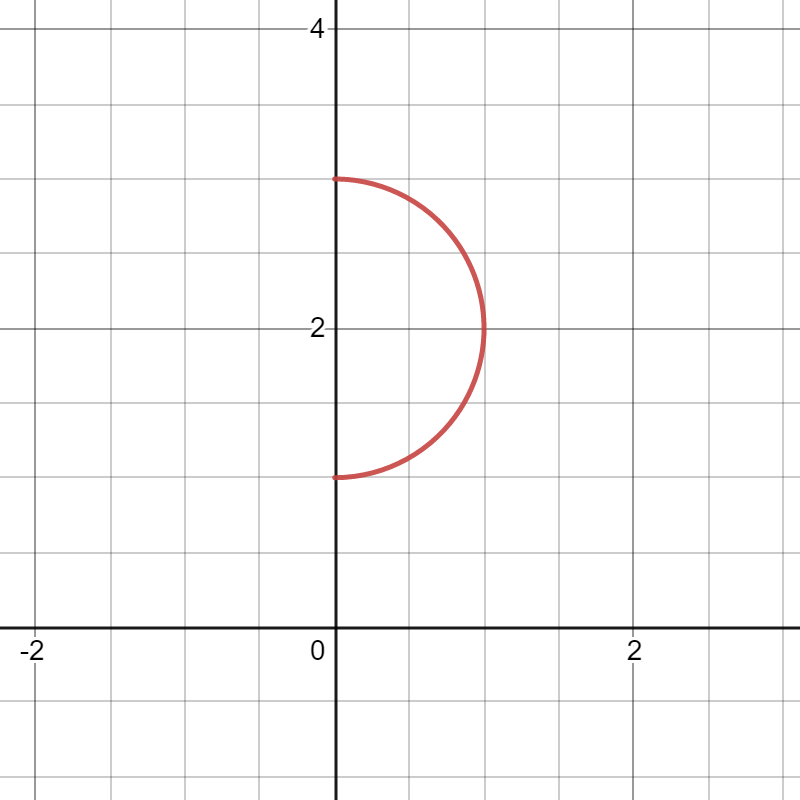
\includegraphics[scale = 0.3]{x-graph}
    
    
    For the function that expresses ${y}$ as a function of ${x}$ i.e
    $${y=h(x)}$$
    The graph is seen below\\    
    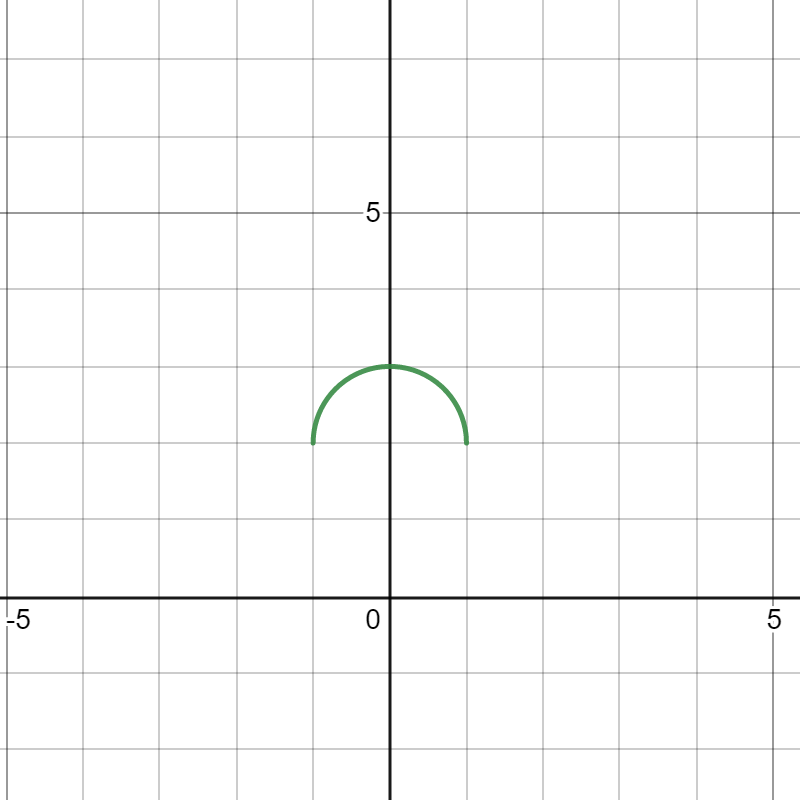
\includegraphics[scale = 0.3]{y-graph}

    \item \textbf{Are there points of the coordinate axes that relate to  ${(0,2)}$ by means of R}\\
    
    Yes all points on the circle has a distance of 1 to the center of the circle at ${(0,2)}$
\end{itemize}
\end{document}
